%\documentclass[12pt]{article}
%\usepackage[a4paper, margin=1in]{geometry} 
%\usepackage{graphicx} 
%\usepackage{hyperref}
%\usepackage{float}
%\usepackage{multicol}
%\usepackage{amsmath}
%\usepackage[ruled]{algorithm2e}
%\usepackage{amssymb}
%\usepackage[font=small, labelfont=bf]{caption}
%
%\begin{document}

%
% Local alignment with DP
%
\subsection{Local alignment with DP}
Dynamic programming can be used to find local alignments.

%
% Requirements
%
\subsubsection*{Requirements}
\begin{itemize}
\item Find all local alignments between two sequences
\item Assign scores to all local alignments
\end{itemize}

%
% Modification of DP for local alignments
%
\subsubsection*{Modification of DP for local alignments}
\begin{itemize}
\item The minimum alignment score must be 0
\item Some entries of the score matrix should be negative
\item Backtracking also needs to be modified
\end{itemize}

%
% Update rule of DP cells
%
\subsubsection*{Update rule of DP cells}
\begin{align*}
H_{i,j}^{(0)} &= H_{i-1,j} - g &(vertical) \\
H_{i,j}^{(1)} &= H_{i,j-1} - g	&(horizontal) \\
H_{i,j}^{(2)} &= H_{i-1,j-1} + R_{a,b} &(diagonal) \\
H_{i,j}^{(2)} &= 0 &(minimum score)
\end{align*}

%
% Example of cell udpate
%
\subsubsection*{Example of cell udpate}
\begin{multicols}{2}
\begin{figure}[H]
  \centering
      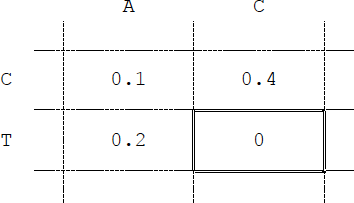
\includegraphics[width=0.3\textwidth]{fig04/local_alignment_cell_update.png}
\end{figure}

\noindent Scoring scheme: \\ 
\null \quad Match: 0.5 \\ 
\null \quad Mismatch: -0.3 \\ 
\null \quad Gap penalty: 0.5

\end{multicols} 

\begin{align*}
H_{i,j}^{(0)} &=  -0.1 &\hfill &(vertical) \\
H_{i,j}^{(1)} &= -0.3 &\hfill &(horizontal) \\
H_{i,j}^{(2)} &= -0.2 &\hfill &(diagonal) \\
H_{i,j}^{(2)} &= 0 & \checkmark &(minimum score)
\end{align*}
\medskip 

%
% Backtracking 
%
\subsubsection*{Backtracking for local alignments}
It starts from the cells with the maximum score instead of the right bottom cell.

\begin{itemize}
\item Start cells: cells with the maximum score 
\item End cells: cells with 0
\end{itemize}

\noindent
\textbf{N.B.} the end cell with score 0 should not be included in the alignment.

%
% Example of backtracking
%
\subsubsection*{Example of backtracking}

\begin{figure}[H]
  \centering
      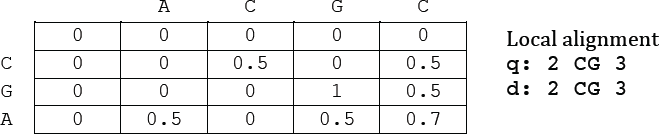
\includegraphics[width=0.7 \textwidth]{fig04/local_alignment_backtrack.png}
\end{figure}

\medskip 

%
% Pseudo-code of local alignment with DP
%
\subsubsection*{Pseudo-code of updating DP table for local alignment}
The cells in the first row and the first column are initialized with 0.

\begin{algorithm}[H]
  \SetKwInOut{HAB}{$\mathrm{H_{i,j}}$}
  \SetKwInOut{RAB}{$\mathrm{R_{a,b}}$}
  \SetKwInOut{G}{$\mathrm{g}$}
  \SetKwData{dRAB}{$\mathrm{R_{a,b}}$}
  \SetKwData{dG}{$\mathrm{g}$}
  
  \BlankLine
    
  \HAB{Dynamic programming table}
  \RAB{Match/mismatch scores}
  \G{Gap penalty}
  
  \BlankLine \BlankLine
  
  \tcp{Initialization}
  \For{$i \leftarrow 0$ \KwTo $m$}{
    $\mathrm{H_{i,0}}$ $\leftarrow$ $\mathbf{0} $\;
  }
  \For{$j \leftarrow 1$ \KwTo $n$}{
    $\mathrm{H_{0,j}}$ $\leftarrow$ $\mathbf{0} $\;
  }
  
  \BlankLine \BlankLine
    
  \tcp{Main loop for table update}
  \For{$i \leftarrow 1$ \KwTo $m$}{
    \For{$j \leftarrow 1$ \KwTo $n$}{
      $\mathrm{H_{i,j}}$ $\leftarrow$ $max(\mathrm{\mathbf{0}, H_{i-1,j}} - \dG, \mathrm{H_{i,j-1}} - \dG, \mathrm{H_{i-1,j-1}}$ + \dRAB)\;
    }
  }
  
  \SetAlgoRefName{\thesection.1}
  \caption{Update dynamic programming table for global alignment}

\end{algorithm}

%
% Exercise \thesection.1
%
\subsubsection*{Exercise \thesection.1}
	
Use DP to find a local alignment.

\begin{multicols}{2}
\begin{figure}[H]
  \centering
      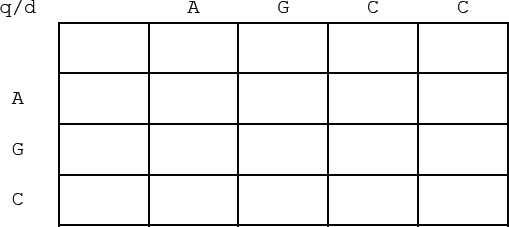
\includegraphics[width=0.4\textwidth]{fig04/local_alignment_exercise.png}
\end{figure}

\noindent Scoring scheme: \\ 
\null \quad Match: 0.2 \\ 
\null \quad Mismatch: -0.2 \\ 
\null \quad Gap penalty: 0.2

\end{multicols} 

\bigskip 

%\end{document}
